\documentclass[11pt,a4paper,oneside,german]{article}
\pagestyle{plain}
\usepackage[ngerman]{babel}
\usepackage[utf8]{inputenc}

\usepackage{geometry}
\geometry{a4paper,left=40mm,right=30mm, top=3.5cm, bottom=2.5cm}
\usepackage{graphicx}
\usepackage{hyperref}
\usepackage{float}
\usepackage{wrapfig}

\title{Praktikumsbericht Data Science 1}
\author{Robin Mayer, Nils Nover, Mariella Zunker}
\date{\today}

\begin{document}
	\maketitle
	
	\begin{figure}[h]
		\centering
		
\includegraphics[width=10.5cm]{uniemblem.jpg}		
	\end{figure}
	
	\newpage
	
	\tableofcontents
	
	\section{Fragestellung und Auswahl der Datensätze}
	
	Die Frage der Schädlichkeit von Stickoxiden und deren Zusammenhang mit Dieselfahrzeugen hat in der Vergangenheit die Debatte um die Verkehrswende dominiert. Um einen Überblick darüber zu bekommen, sollten in diesem Projekt Antriebsdaten mit NO2-Werten in Deutschland verglichen werden. \\
	Zur Analyse wurden jahrweise .xlx-Datensätze mit NO2-Werten des Umweltbundesamtes (UBA, Abb. \ref{fig:BeispielNO2}, (1)) sowie .pdf-Dateien des Kraftfahrtbundesamtes (KBA, Abb. \ref{fig:BeispielKFZ}. (2)) genutzt.
	
	\begin{figure}[h!]
		\centering
		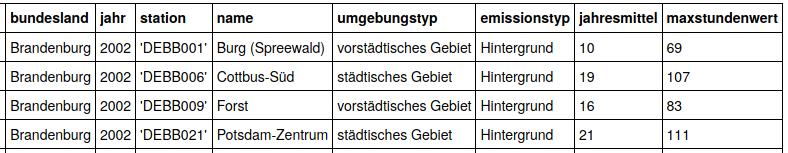
\includegraphics[width=10.5cm]{BeispielNO2.png}
		\caption{Auszug aus dem NO2-Datensatz.}
		\label{fig:BeispielNO2}
	\end{figure}
	
	\begin{figure}[h!]
		\centering
		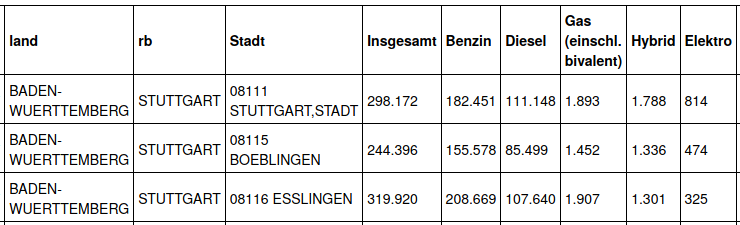
\includegraphics[width=10.5cm]{BeispielKFZ.png}
		\caption{Auszug aus dem KFZ-Datensatz.}
		\label{fig:BeispielKFZ}
	\end{figure}
	
	\section{Datenaufbereitung}
	
	Zur sinnvollen Verarbeitung wurden die .pdf-Dateien ins .xslx-Format konvertiert. Aufgrund der großen Unterschiede der Formate musste manuell viel nachgebessert werden. Die .xlsx-Dateien wurden im Anschluss in ein .csv-Format konvertiert und so eingelesen.\\
	Aufgrund der Verfügbarkeit bestehender Tools wurde für die Auswertung Python mit den Analysetools Pandas sowie Numpy und Matplotlib gewählt und das Jupyter Notebook als übersichtliche IDE genutzt.\\
	Nach dem Einlesen wurden die Datensätze auf Vollständigkeit und Fehler durchsucht. Dabei wurde auf nicht erfasste Datenpunkte sowie offensichtliche Abweichungen wie negative Zahlen geachtet. Zudem wurden alle als String codierten Variablen überprüft und vereinheitlicht. So wurden alle Namen in Großbuchstaben und ohne Umlaute dargestellt, sowie Rechtschreibfehler und Unterschiede in der Darstellung von Doppelnamen korrigiert. Trennzeichen wurden vereinheitlicht und Zahlenwerte als Float gecastet. \\
	Messwerte, für die kein Ort angegeben war, wurden aus dem Datensatz gelöscht, da eine Zuordnung in der verfügbaren Zeit nicht möglich war. Schließlich wurde aus den einzelnen Dateien für jedes Jahr eine Gesamtdatei für alle Jahre erstellt. \\
	Die Aufbereitung der Daten nahm viel Zeit in Anspruch. Mit mehr Kapazitäten hätten Fehlerbehebung und Vervollständigung der Daten noch stärker verfolgt werden können, indem z.B. alle Daten zugeordnet werden oder die Verteilung der Werte genauer betrachtet wird. In Abbildung \ref{fig:Heatmaps} sind beispielhaft einige Daten als Heatmaps dargestellt.
	
	\begin{figure}[h!]
		\centering
		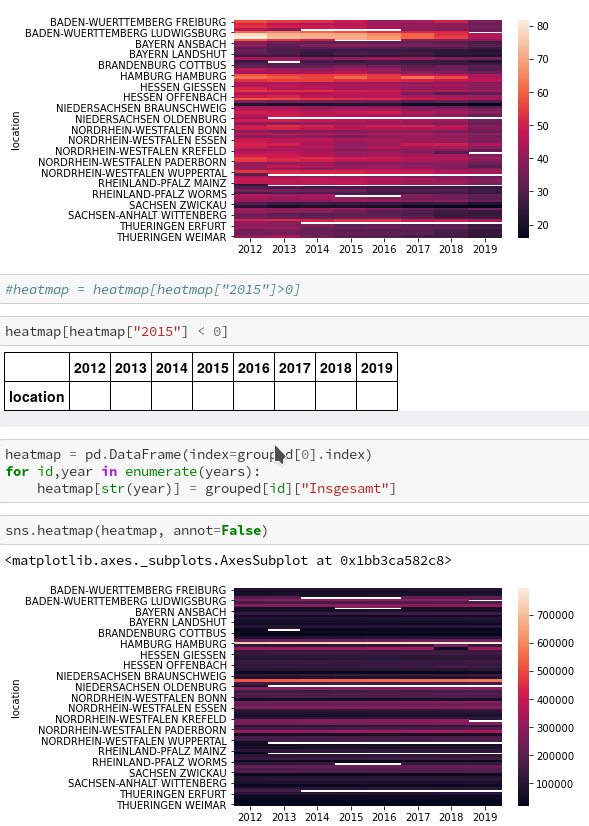
\includegraphics[width=12cm]{Heatmaps.png}
		\caption{Ausschnitt aus den Daten als Heatmaps dargestellt. Links die NO2-Werteentwicklung, rechts die Entwicklung der Autoanzahlen.}
		\label{fig:Heatmaps}
	\end{figure}
	
	\section{Datenauswertung}
	
	\subsection{Betrachtung der beiden Datensätze}
	
	Die Datensätze wurden zuerst isoliert betrachtet. Zur Messung der NO2-Werte existierten Daten aus den Jahren 2002-2019, KfZ-Daten konnten von 2012-2019 genutzt werden. Die  Datensätze enthielten auch Zuordnungen der einzelnen Orte zu verschiedenen Abstufungen der Urbanität wie "vorstädtisches Gebiet", die zur Vereinfachung zu den drei Kategorien "städtisch", "vorstädtisch" sowie "ländlich" zusammengefasst wurden. Für einen ersten Überblick wurden die NO2-Werte über die Zeit geplottet (Abb. \ref{fig:NO2Entwicklung}). In der Tendenz stimmt das Ergebnis mit der Auswertung des UBA (3) überein, die absoluten Werte weisen leichte Abweichungen auf. Dies ist wohl auf die veränderte Einteilung der Orte in die Kategorien zurückzuführen.\\
	
	\begin{figure}[h!]
		\centering
		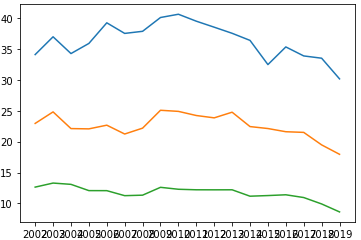
\includegraphics[width=8.5cm]{NO2Entwicklung.png}
		\caption{Entwicklung der NO2-Werte über die Zeit. Blau: Städtisch. Gelb: Vorstädtisch. Grün: Ländlich.}
		\label{fig:NO2Entwicklung}
	\end{figure}
	
	Zur weiteren Analyse wurden die Datensätze im Anschluss zusammengefügt. Dafür wurde pro Jahr und Bundesland überprüft, ob eine Stadt im NO2-Datensatz auch im KfZ-Datensatz existiert und bei Übereinstimmung wurden neue Spalten hinzugefügt. Dieses Merging stellte eine größere Schwierigkeit dar als vermutet, da die Datensätze nicht die gleiche Zuordnung der Werte zu den Orten enthielten. So bezogen sich die Daten des KBA auf die regulären Landkreise, die Messungen des UBA waren jedoch lediglich dem nächsten Ort zugewiesen. Diese Zuordnung führte dazu, dass beim Merging ländliche Gebiete weniger gut zugeordnet werden konnten als größere Städte (Abb. \ref{fig:Kategorien}).\\
	
	\begin{wrapfigure}{r}{0.4\textwidth}
		\vspace{-20pt}
		\begin{center}
			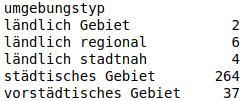
\includegraphics[width=4.5cm]{Kategorien.jpg}
			\caption{Anzahl an Orten in den Kategorien, die zugeordnet werden konnten.}
			\label{fig:Kategorien}
		\end{center}
		\vspace{-20pt}
	\end{wrapfigure}
	
	Zudem ist zu beachten, dass einige Städte in den Datensätzen mehrfach vorkommen (z.B. Weimar Schwanseestr. und Weimar Steubenstr.). Hier wurde zur Vereinfachung der Mittelwert dieser Stationen verwendet. Das Merging beanspruchte einen Großteil der Zeit des gesamten Projektes und konnte dennoch nicht die angestrebte Vollständigkeit erreichen. Wäre mehr Zeit vorhanden, hätten noch mehr Versuche angestrengt werden können, alle Städte in den beiden Datensätzen zuzuordnen. Möglich wäre dabei, die Orte eindeutig mithilfe eines Karten-Tools zu ermitteln. Auch auf Ausreißer hätte mehr geachtet werden können. Zudem wäre es noch interessant gewesen, die zeitliche Entwicklung in den Daten zu betrachten und diese in gesellschaftliche Kontexte zu setzen, wie z.B. Gesetzesänderungen, Umweltzonen und lokale Unterschiede.
	
	\subsection{Betrachtung der Werte und lineare Regression}
	
	Im Anschluss an die Zuordnung wurden die NO2-Werte gegen die Fahrzeugzahlen aufgetragen. Dabei konnte bereits ein grober Trend erkannt werden. Mithilfe linearer Regression wurde versucht, den Zusammenhang genauer zu beschreiben (\ref{fig:linreginsgesamt}). Außerdem zeigten sich im Bereich der Fahrzeugzahlen einige extreme Ausreißer.
	
	\begin{figure}[h!]
		\centering
		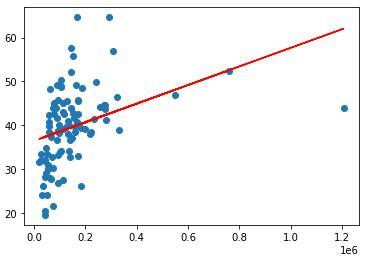
\includegraphics[width=6.5cm]{linreginsgesamt.jpg}
		\caption{NO2-Werte in Abhängigkeit der Fahrzeugzahlen.}
		\label{fig:linreginsgesamt}
	\end{figure}
	
	Das Ergebnis wurde anschließend mithilfe von drei Error-Parametern evaluiert. Dabei zeigte sich ein mittlerer absoluter Fehler von 6,21, ein MSE von 66,82 sowie ein R2-Score von 0,13. Die gefundene Regressionsgerade beschreibt den gefundenen Zusammenhang somit eher weniger gut. \\
	Die Auswertung wurde schließlich noch einmal unter Ausschluss der Ausreißer durch-geführt, brachte jedoch keine nennenswerte Besserung. \\
	Dann wurde der Anteil an Dieselfahrzeugen betrachtet und gegen die NO2-Werte aufgetragen. Eine grobe Betrachtung des Plots ließ zunächst auf eine eher zufällige Verteilung mit geringfügiger linearer Tendenz schließen. Auch durch lineare Regression konnte hierbei kein starker Zusammenhang festgestellt werden (Abb. \ref{fig:linregdieselanteil}).
	
	\begin{figure}[H]
		\centering
		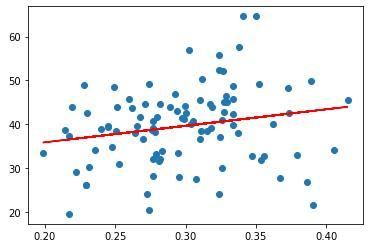
\includegraphics[width=6.5cm]{linregdieselanteil.jpg}
		\caption{NO2-Werte in Abhängigkeit des Dieselanteils.}
		\label{fig:linregdieselanteil}
	\end{figure}
	
	Die Evaluation ergab hierbei einen absoluten durchschnittlichen Fehler von 6,64, einen MSE von 74,04 sowie einen R2-Score von 0,04, und lässt darauf schließen, dass hier kein sinnvoller Erkenntnisgewinn durch die lineare Regression geschaffen wurde.
	
	\subsection{Nicht-lineare Regression}
	
	Die Größe des Stadtgebietes und physikalische Eigenschaften der Gase wie Diffusion könnten dafür sorgen, dass sich der Zusammenhang mit einer Wachstumskurve anstelle einer Gerade genauer beschreiben lässt. Die Auslastung der Straßen ist je nach Größe auf einen bestimmten Verkehrsdurchfluss begrenzt. Neue Fahrzeuge in der Stadt sorgen hier also nicht gleichzeitig für einen hören NO2 Wert. Daher ist es möglich, dass eine Sättigungskurve die NO2-Entwicklung besser beschreibt. Es wurde also noch eine nicht-lineare Regressionsanalyse durchgeführt (Abb. \ref{fig:nonlinreg}).
	
	\begin{figure}[H]
	\centering
	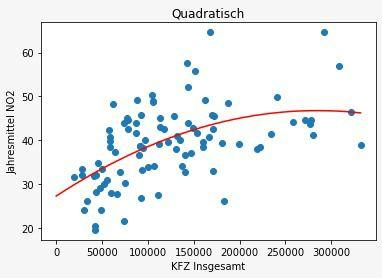
\includegraphics[width=6.5cm]{nonlinreg.jpg}
	\caption{Nicht-lineare Regression des Zusammenhangs von Fahrzeugzahlen und NO2-Werten.}
	\label{fig:nonlinreg}
	\end{figure}
	
	\section{Diskussion}
	
	Der Zusammenhang zwischen NO2-Werten und Fahrzeugzahlen wurde durch die Daten zwar gut gezeigt, doch die Regressionsanalyse zeigt, dass für eine genaue Beschreibung zusätzliche Daten benötigt werden. So ist zweifelhaft, ob Autos auch tatsächlich nur an ihrem Meldeort gefahren werden. Gewerbe, die alle Fahrzeuge in einer Stadt melden, können die Ergebnisse verzerren. Es sollten Fahrzeugdaten verwendet werden, die an einer Stelle nachgewiesen wurden. Um statistische Sicherheit zu erlangen, wäre zudem ein Hypothesentest notwendig. \\
	Bei der Analyse der Dieselfahrzeuge wurde kein zuverlässiger Zusammenhang gefunden. Allerdings kann die Einteilung in Diesel/Nicht-Diesel hierbei als zu grob betrachtet werden. \\
	Insgesamt war vor allem die Datenaufbereitung und das Merging der Datensätze mit Schwierigkeiten verbunden. Mit mehr Zeit wäre es vielleicht möglich gewesen, sich die zeitliche Entwicklung anzusehen. Die Ergebnisse zeigten zwar sinkende NO2-Werte über die Zeit, doch von genauerem Interesse wären auch lokale Unterschiede wie Umweltzonen oder Ballungsräume. \\
	Auch der Vergleich von urbanen und ländlichen Gebieten konnte aufgrund der Herausforderungen bei der Fusion der Datensätze nicht gezogen werden. Wenn die Städte eindeutig zuzuordnen wären, wäre noch eine genauere Analyse von Einflussfaktoren möglich. \\
	
	\section{Quellen}
	
	(1) https://www.umweltbundesamt.de/themen/luft/luftschadstoffe/stickstoffoxide\\
	(2) https://www.kba.de/DE/Statistik/Fahrzeuge/Bestand/ZulassungsbezirkeGemei-nden/zulassungsbezirke\_node.html\\
	(3) https://www.umweltbundesamt.de/themen/luft/daten-karten/entwicklung-der-luftqualitaet\#entwicklung-der-luftqualitat-in-deutschland
	
	
	
\end{document}